\documentclass[12pt]{article}
\usepackage{parskip}
\usepackage[letterpaper, margin=1in]{geometry}
\usepackage{graphicx}
\usepackage{amsmath}
\usepackage{enumitem}
\graphicspath{{./images/}}
\title{ELECENG 3EJ4 Lab 1}
\author{Raeed Hassan \\ hassam41 \\ McMaster University}
\begin{document}
\maketitle
\pagebreak
\begin{itemize}
    \section*{Part 1}
    \item [\textbf{Q1.}]
    The data from these plots indicate that the NPN (in both simulation and in measured experimentation) operates in the active region for $V_{CC}$ between 0.5 V to 5 V when the value of $V_E$ is between -5 V and -1 V. The $i_c-V_{CE}$ characteristics of the NPN in this region is generally linear, which is the expected behaviour of a BJT in the active region. The plots for simulated and measured $I_C$ vs. $V_{CE}$ characteristics are shown in Figure \ref{fig:q1}.
    \begin{figure}[ht]
        \centering
        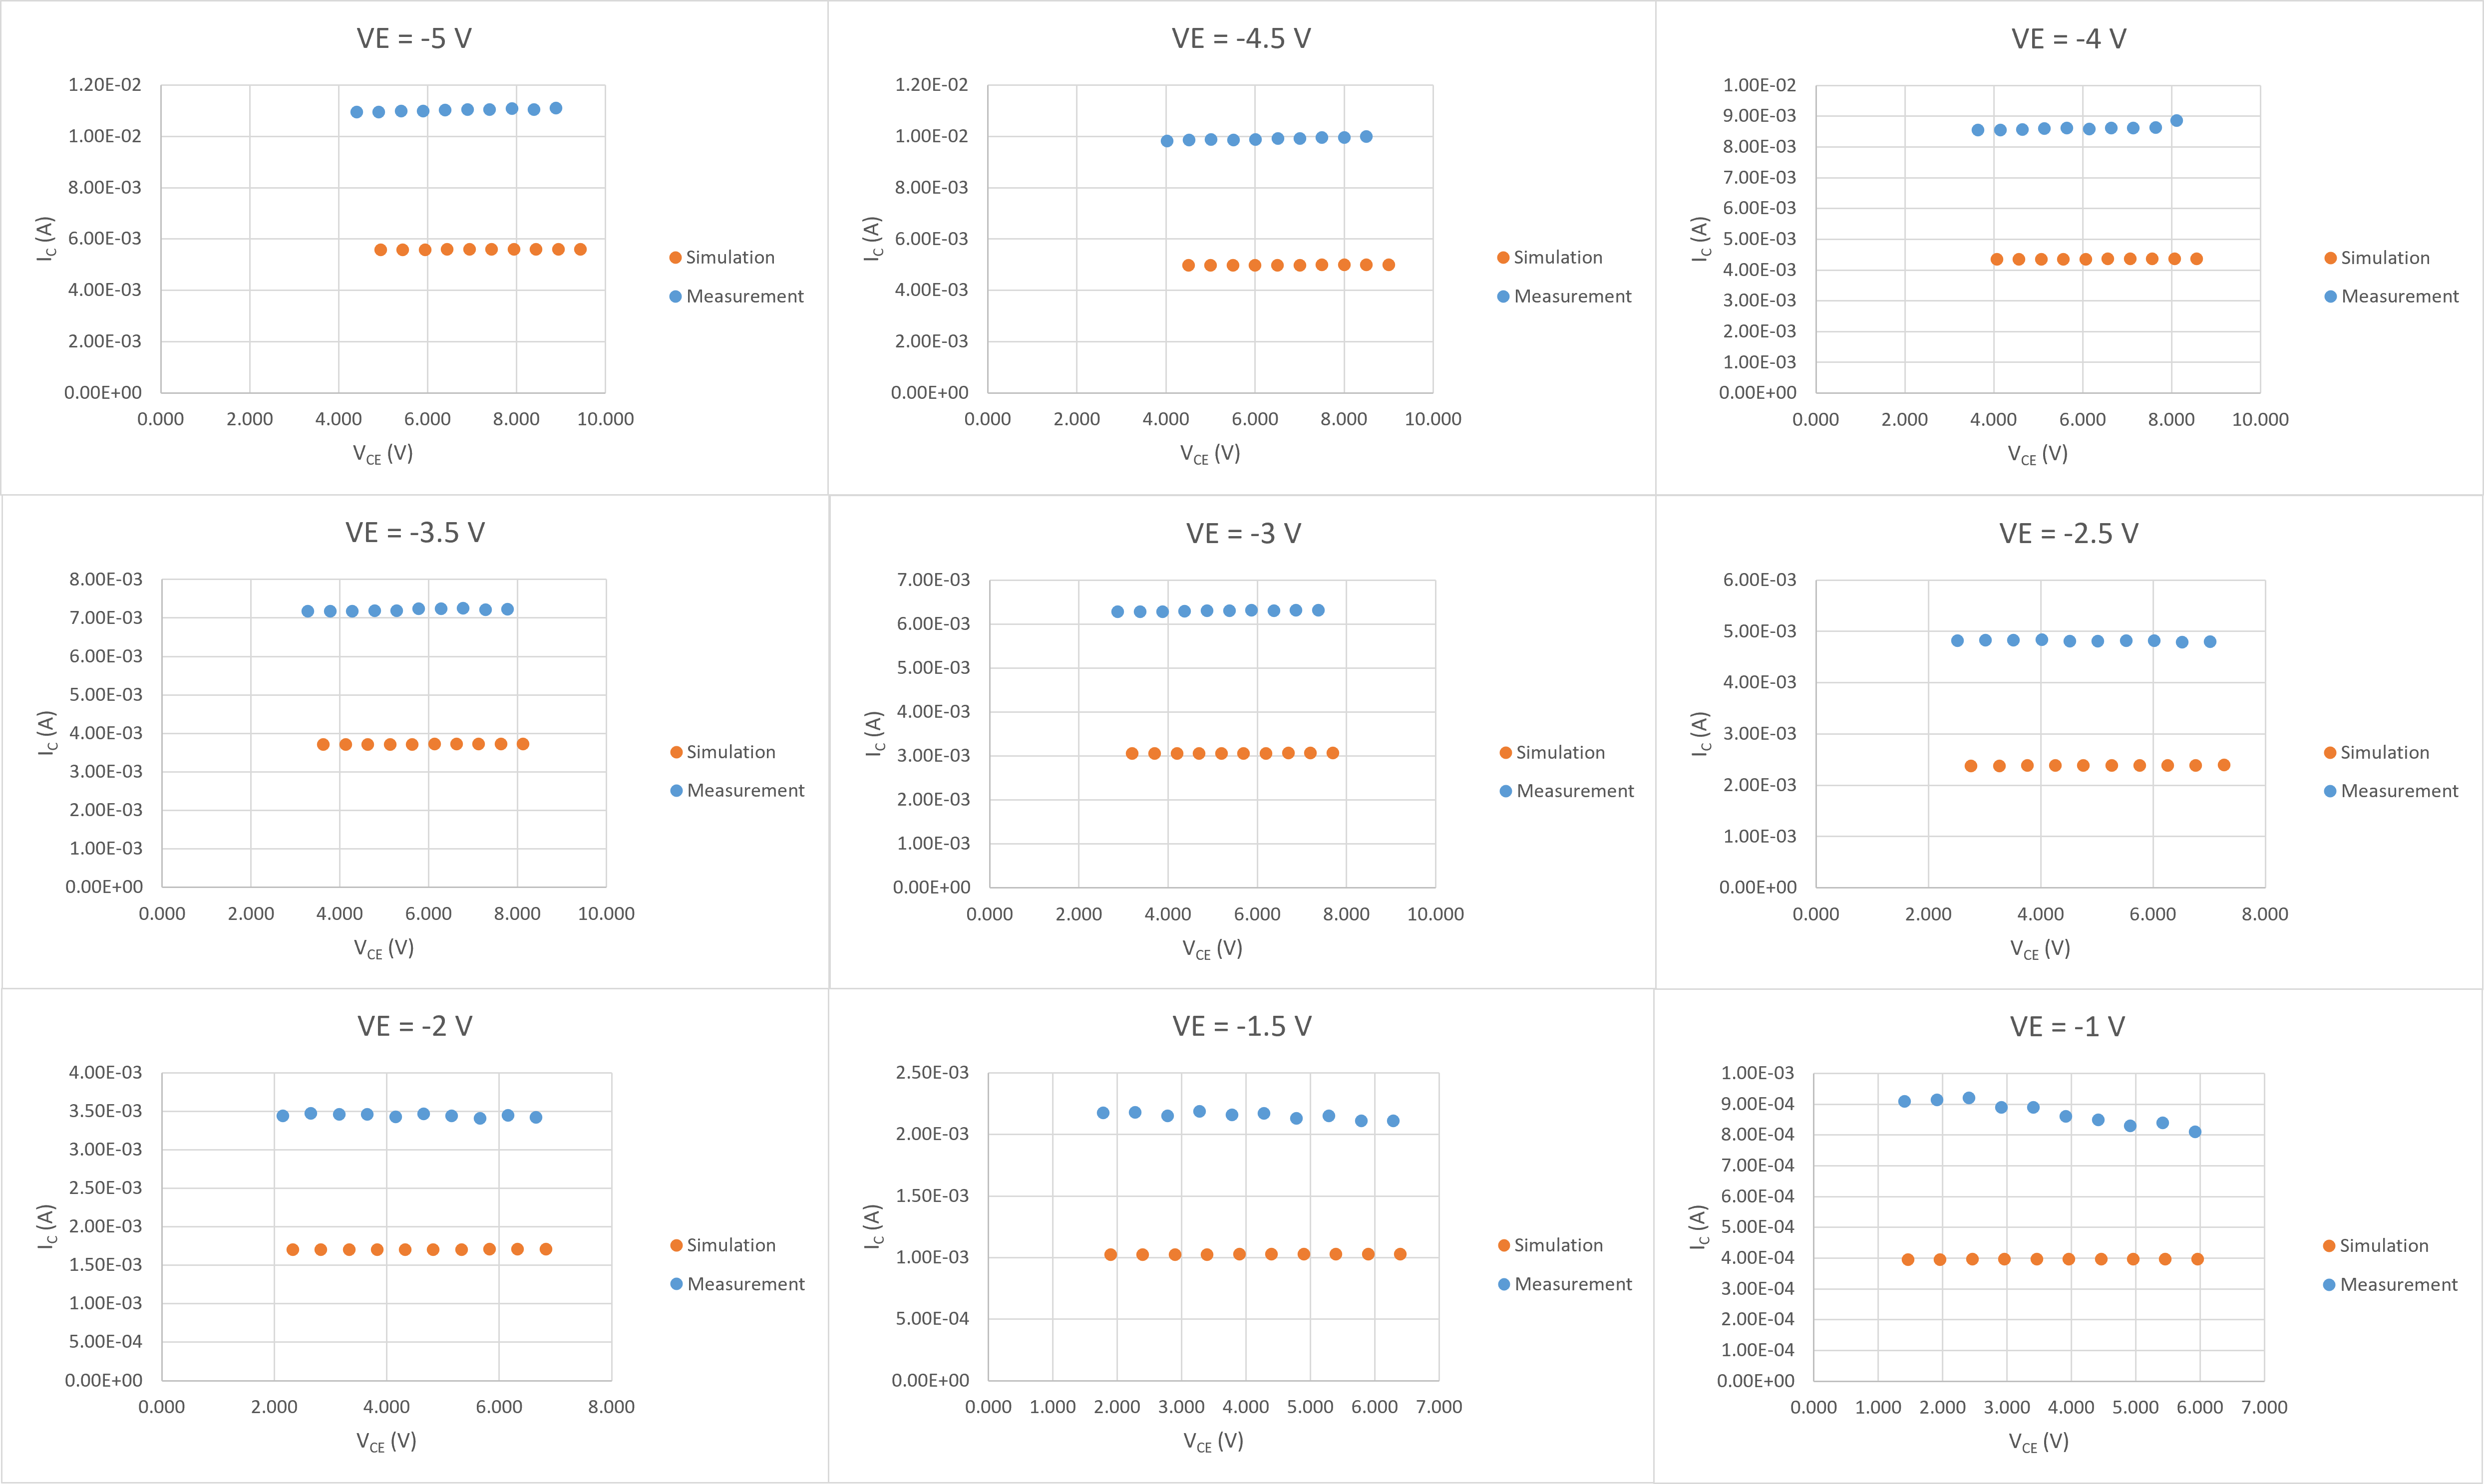
\includegraphics[width=\textwidth]{Q1.png}
        \caption{$I_C$ vs. $V_{CE}$ for $V_{CC}$ between 0.5 V and 5 V at various values of $V_E$ for NPN}
        \label{fig:q1}
    \end{figure}
    \item [\textbf{Q2.}]
    The values determined for $\beta$, $V_{BE_{on}}$, $|V_A|$, $g_m$, $r_{\pi}$, and $r_o$ in reference $V_{CE}$ in simulation and in measured experiments were generally found to be similar to the expected values for these characteristics. This was verified by comparing these values with the parameters in the SPICE model for the part provided by the manufacturer. The plots for the simulated and measured characters are shown in Figure \ref{fig:q2}.
    \begin{figure}[ht]
        \centering
        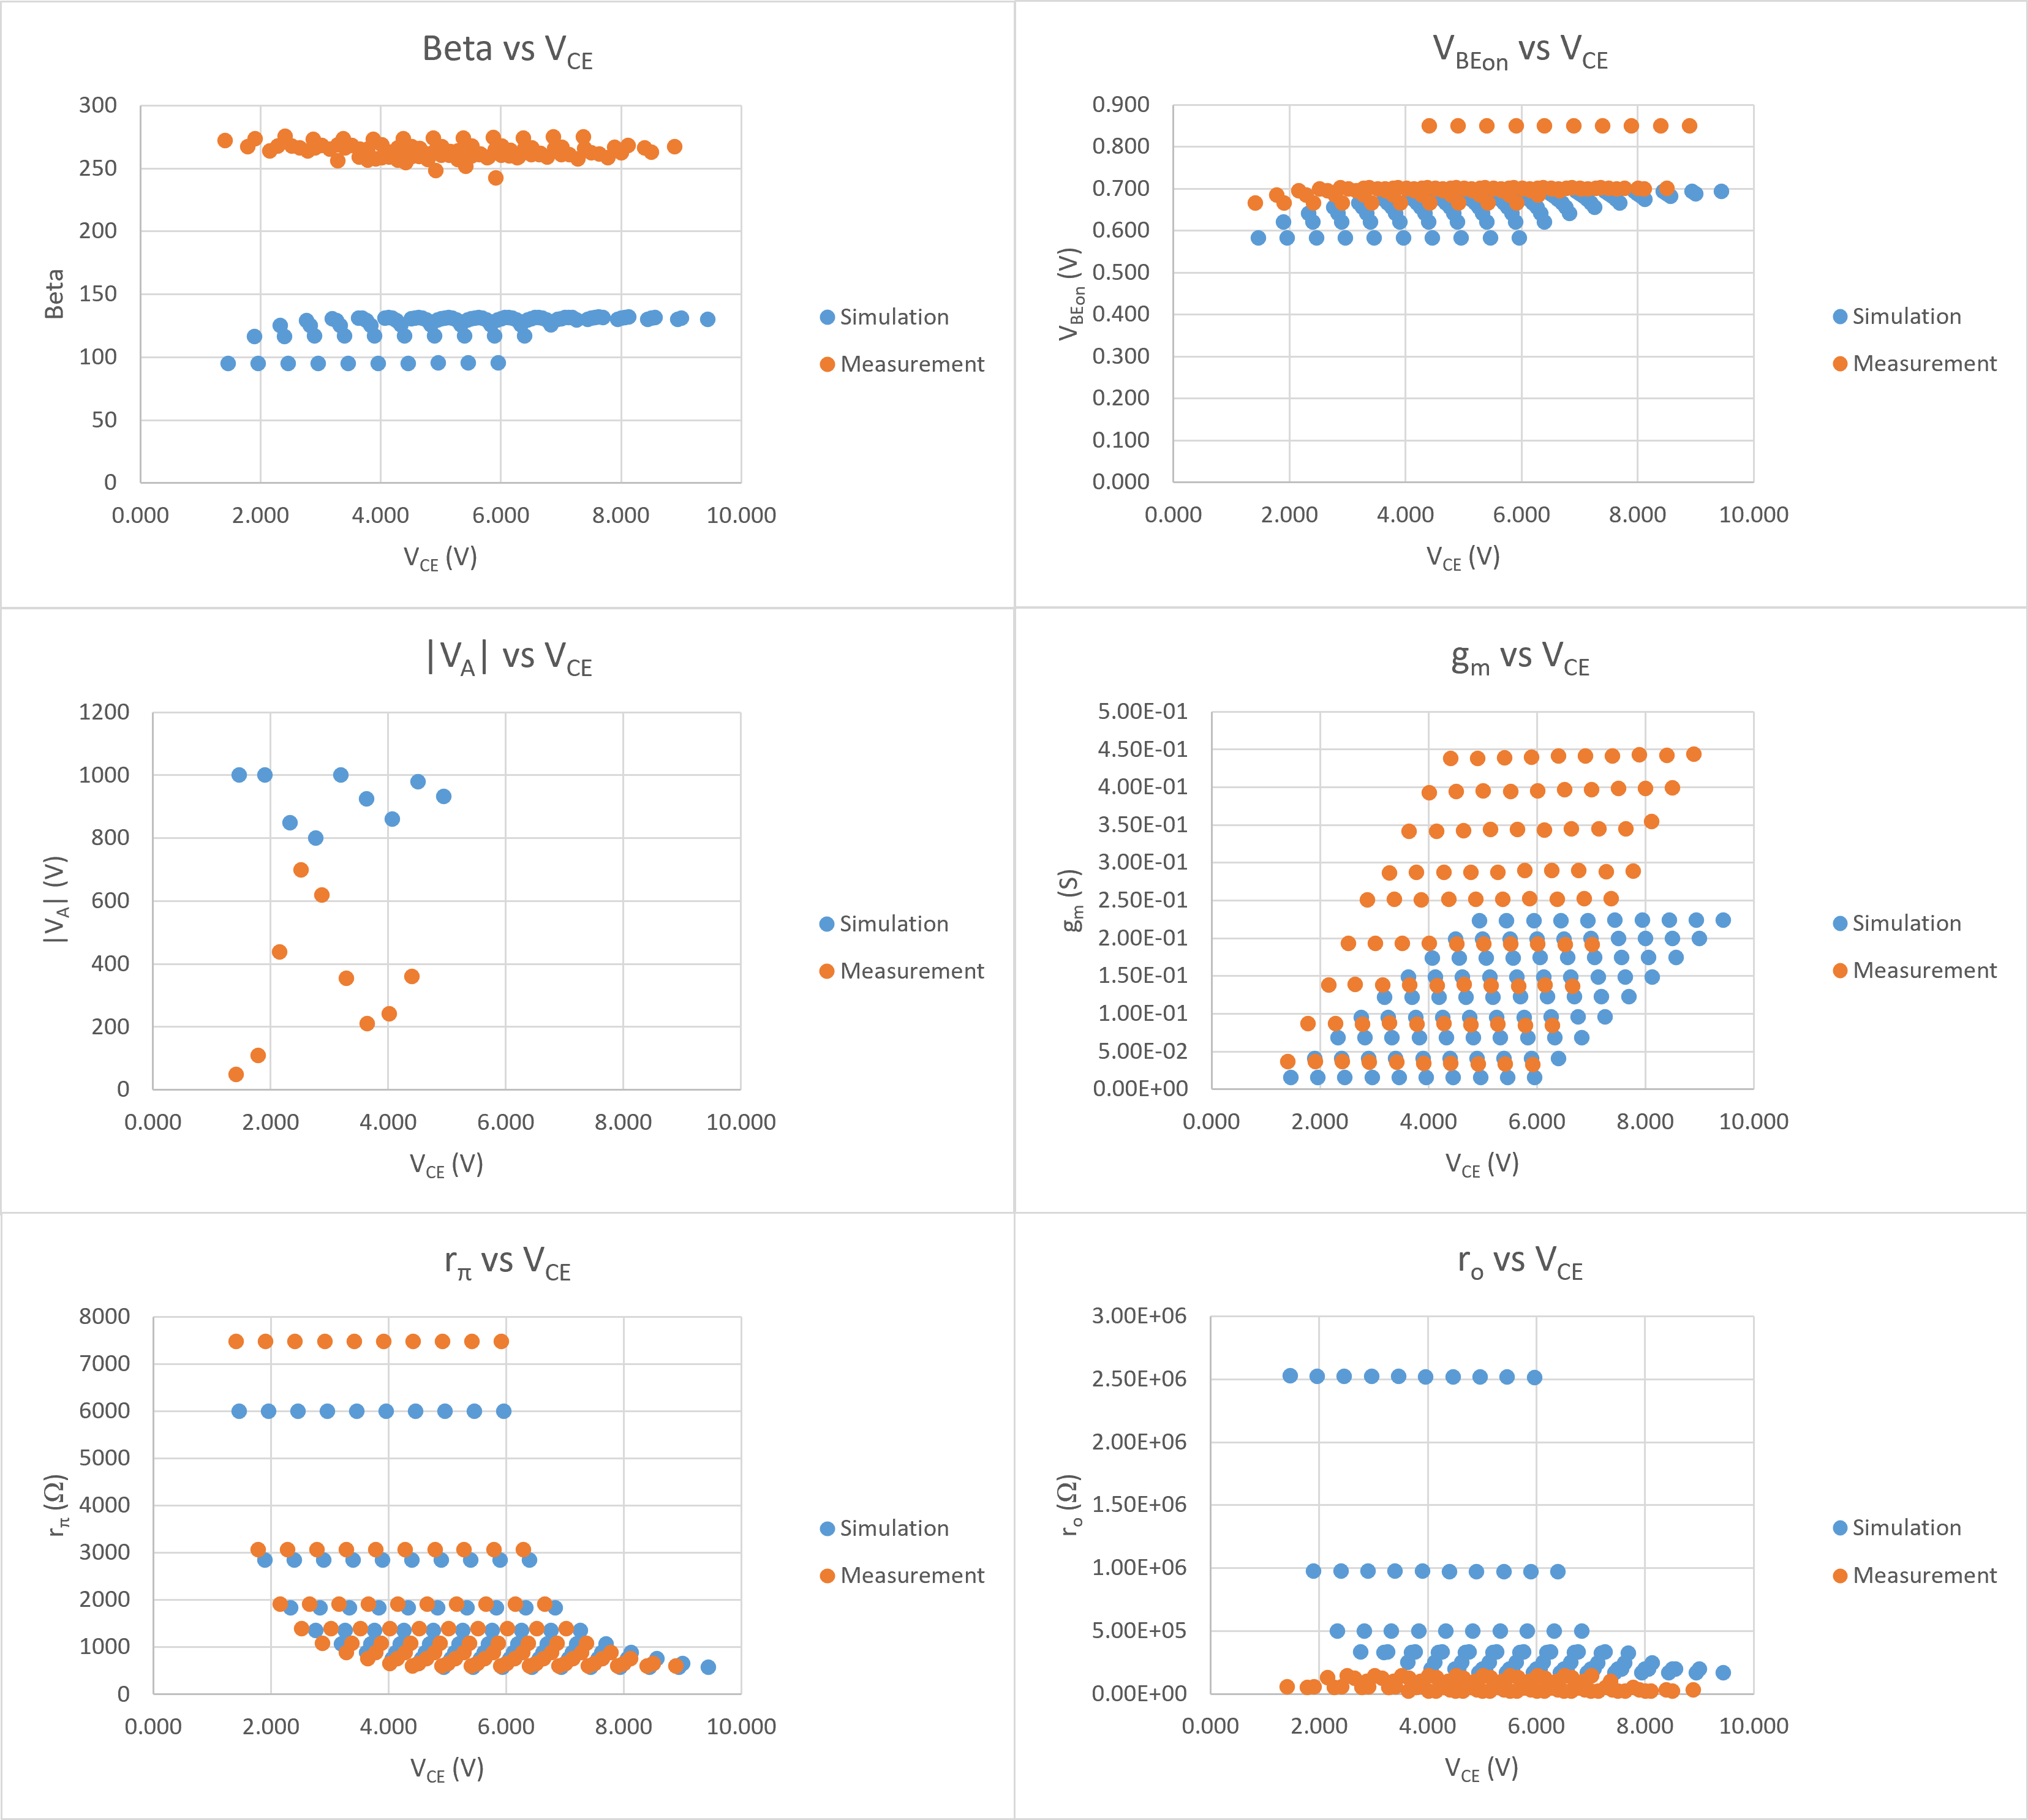
\includegraphics[width=\textwidth]{Q2.png}
        \caption{$\beta$, $V_{BE_{on}}$, $|V_A|$, $g_m$, $r_{\pi}$, $r_o$ vs $V_{CE}$ plots for NPN}
        \label{fig:q2}
    \end{figure} \pagebreak
    \item [\textbf{Q3.}]
    In general, there were no discrepancies between the simulated and measured data; they displayed the similar behaviours in the majority of plots in Figures \ref{fig:q1} and \ref{fig:q2}. The only differences were generally slight shifts between the simulated and measured data, which can be due to a number of factors such as tolerances in the physical components and inaccuracies in the measurements taken by the AD2 board. \pagebreak
    \section*{Part 2}
    \item [\textbf{Q4.}]
    The data from these plots indicate that the PNP (in both simulation and in measured experimentation) operates in the active region for $V_{CC}$ between -5 V to -0.5 V when the value of $V_E$ is between 5 V and 1 V. The $i_c-|V_{CE}|$ characteristics of the PNP in this region is generally linear, which is the expected behaviour of a BJT in the active region. he plots for simulated and measured $I_C$ vs. $|V_{CE}|$ characteristics are showed in Figure \ref{fig:q4}. \\
    \begin{figure}[ht]
        \centering
        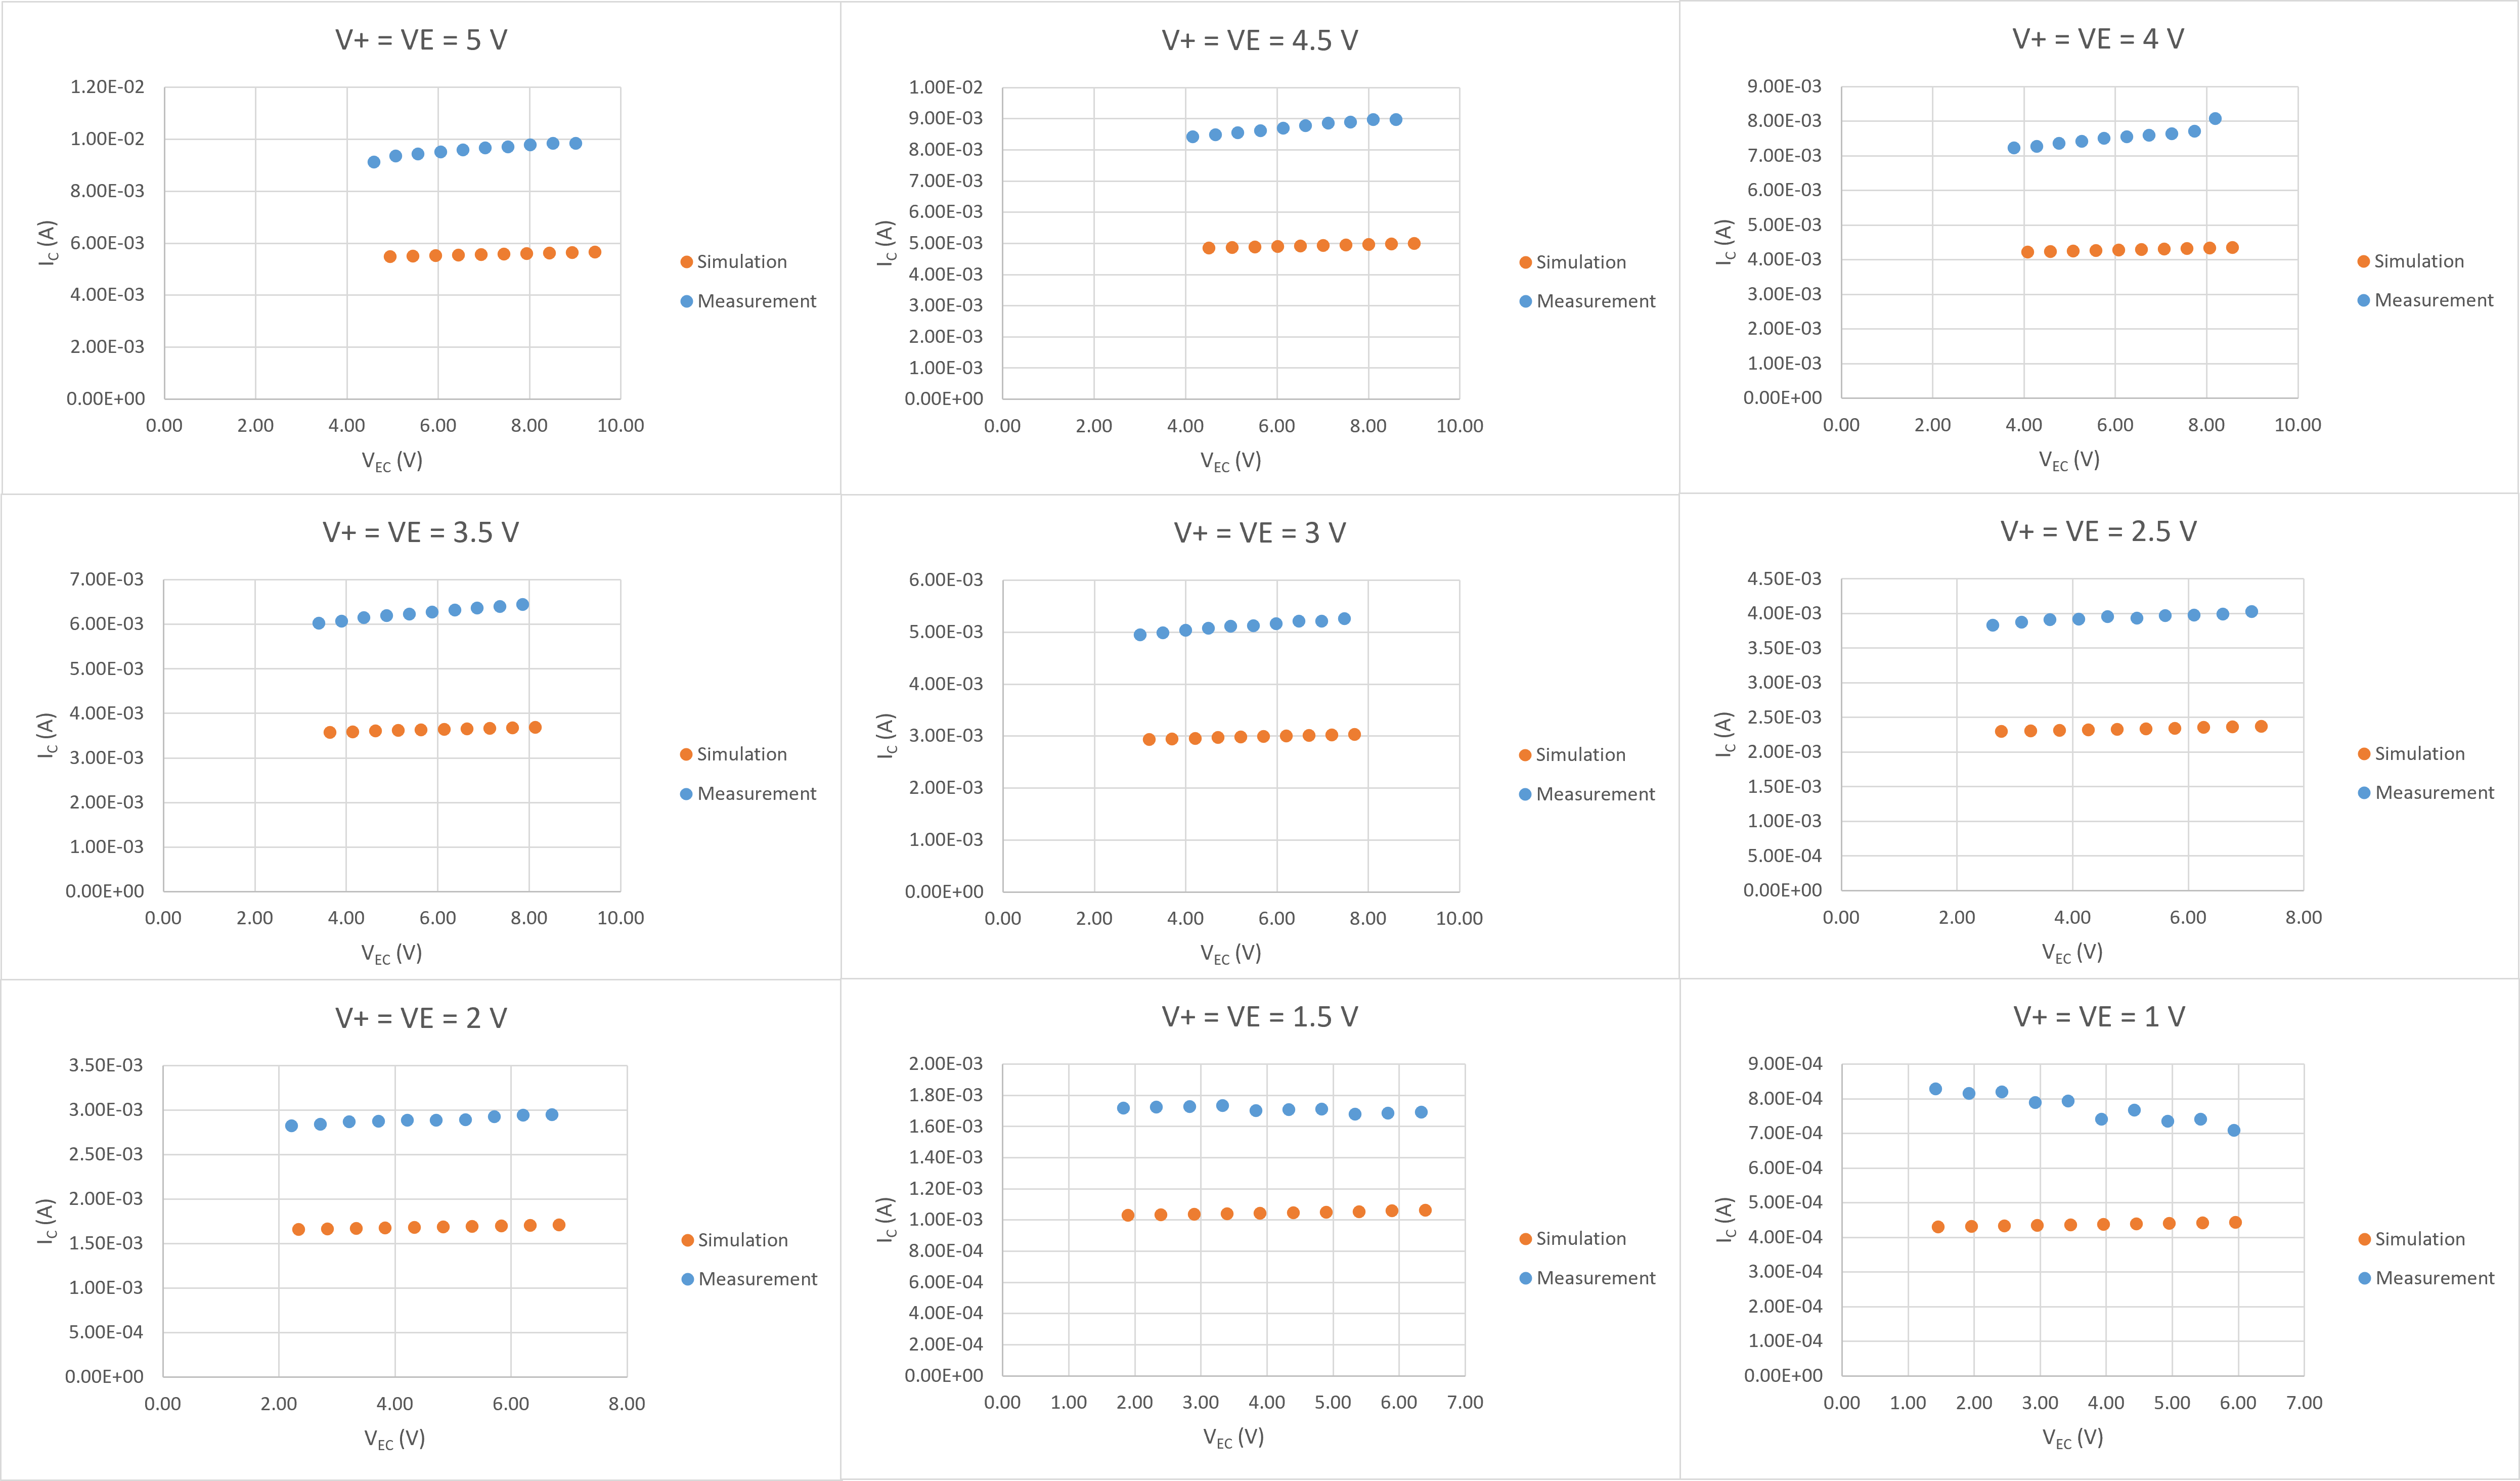
\includegraphics[width=\textwidth]{Q4.png}
        \caption{$I_C$ vs. $|V_{CE}|$ for $V_{CC}$ between -0.5 V and -5 V at various values of $V_E$ for PNP}
        \label{fig:q4}
    \end{figure}
    \item [\textbf{Q5.}]
    The values determined for $\beta$, $V_{EB_{on}}$, $|V_A|$, $g_m$, $r_{\pi}$, and $r_o$ in reference $|V_{CE}|$ in simulation and in measured experiments were generally found to be similar to the expected values for these characteristics. This was verified by comparing these values with the parameters in the SPICE model for the part provided by the manufacturer. The plots for the simulated and measured characters are shown in Figure \ref{fig:q5}.
    \begin{figure}[ht]
        \centering
        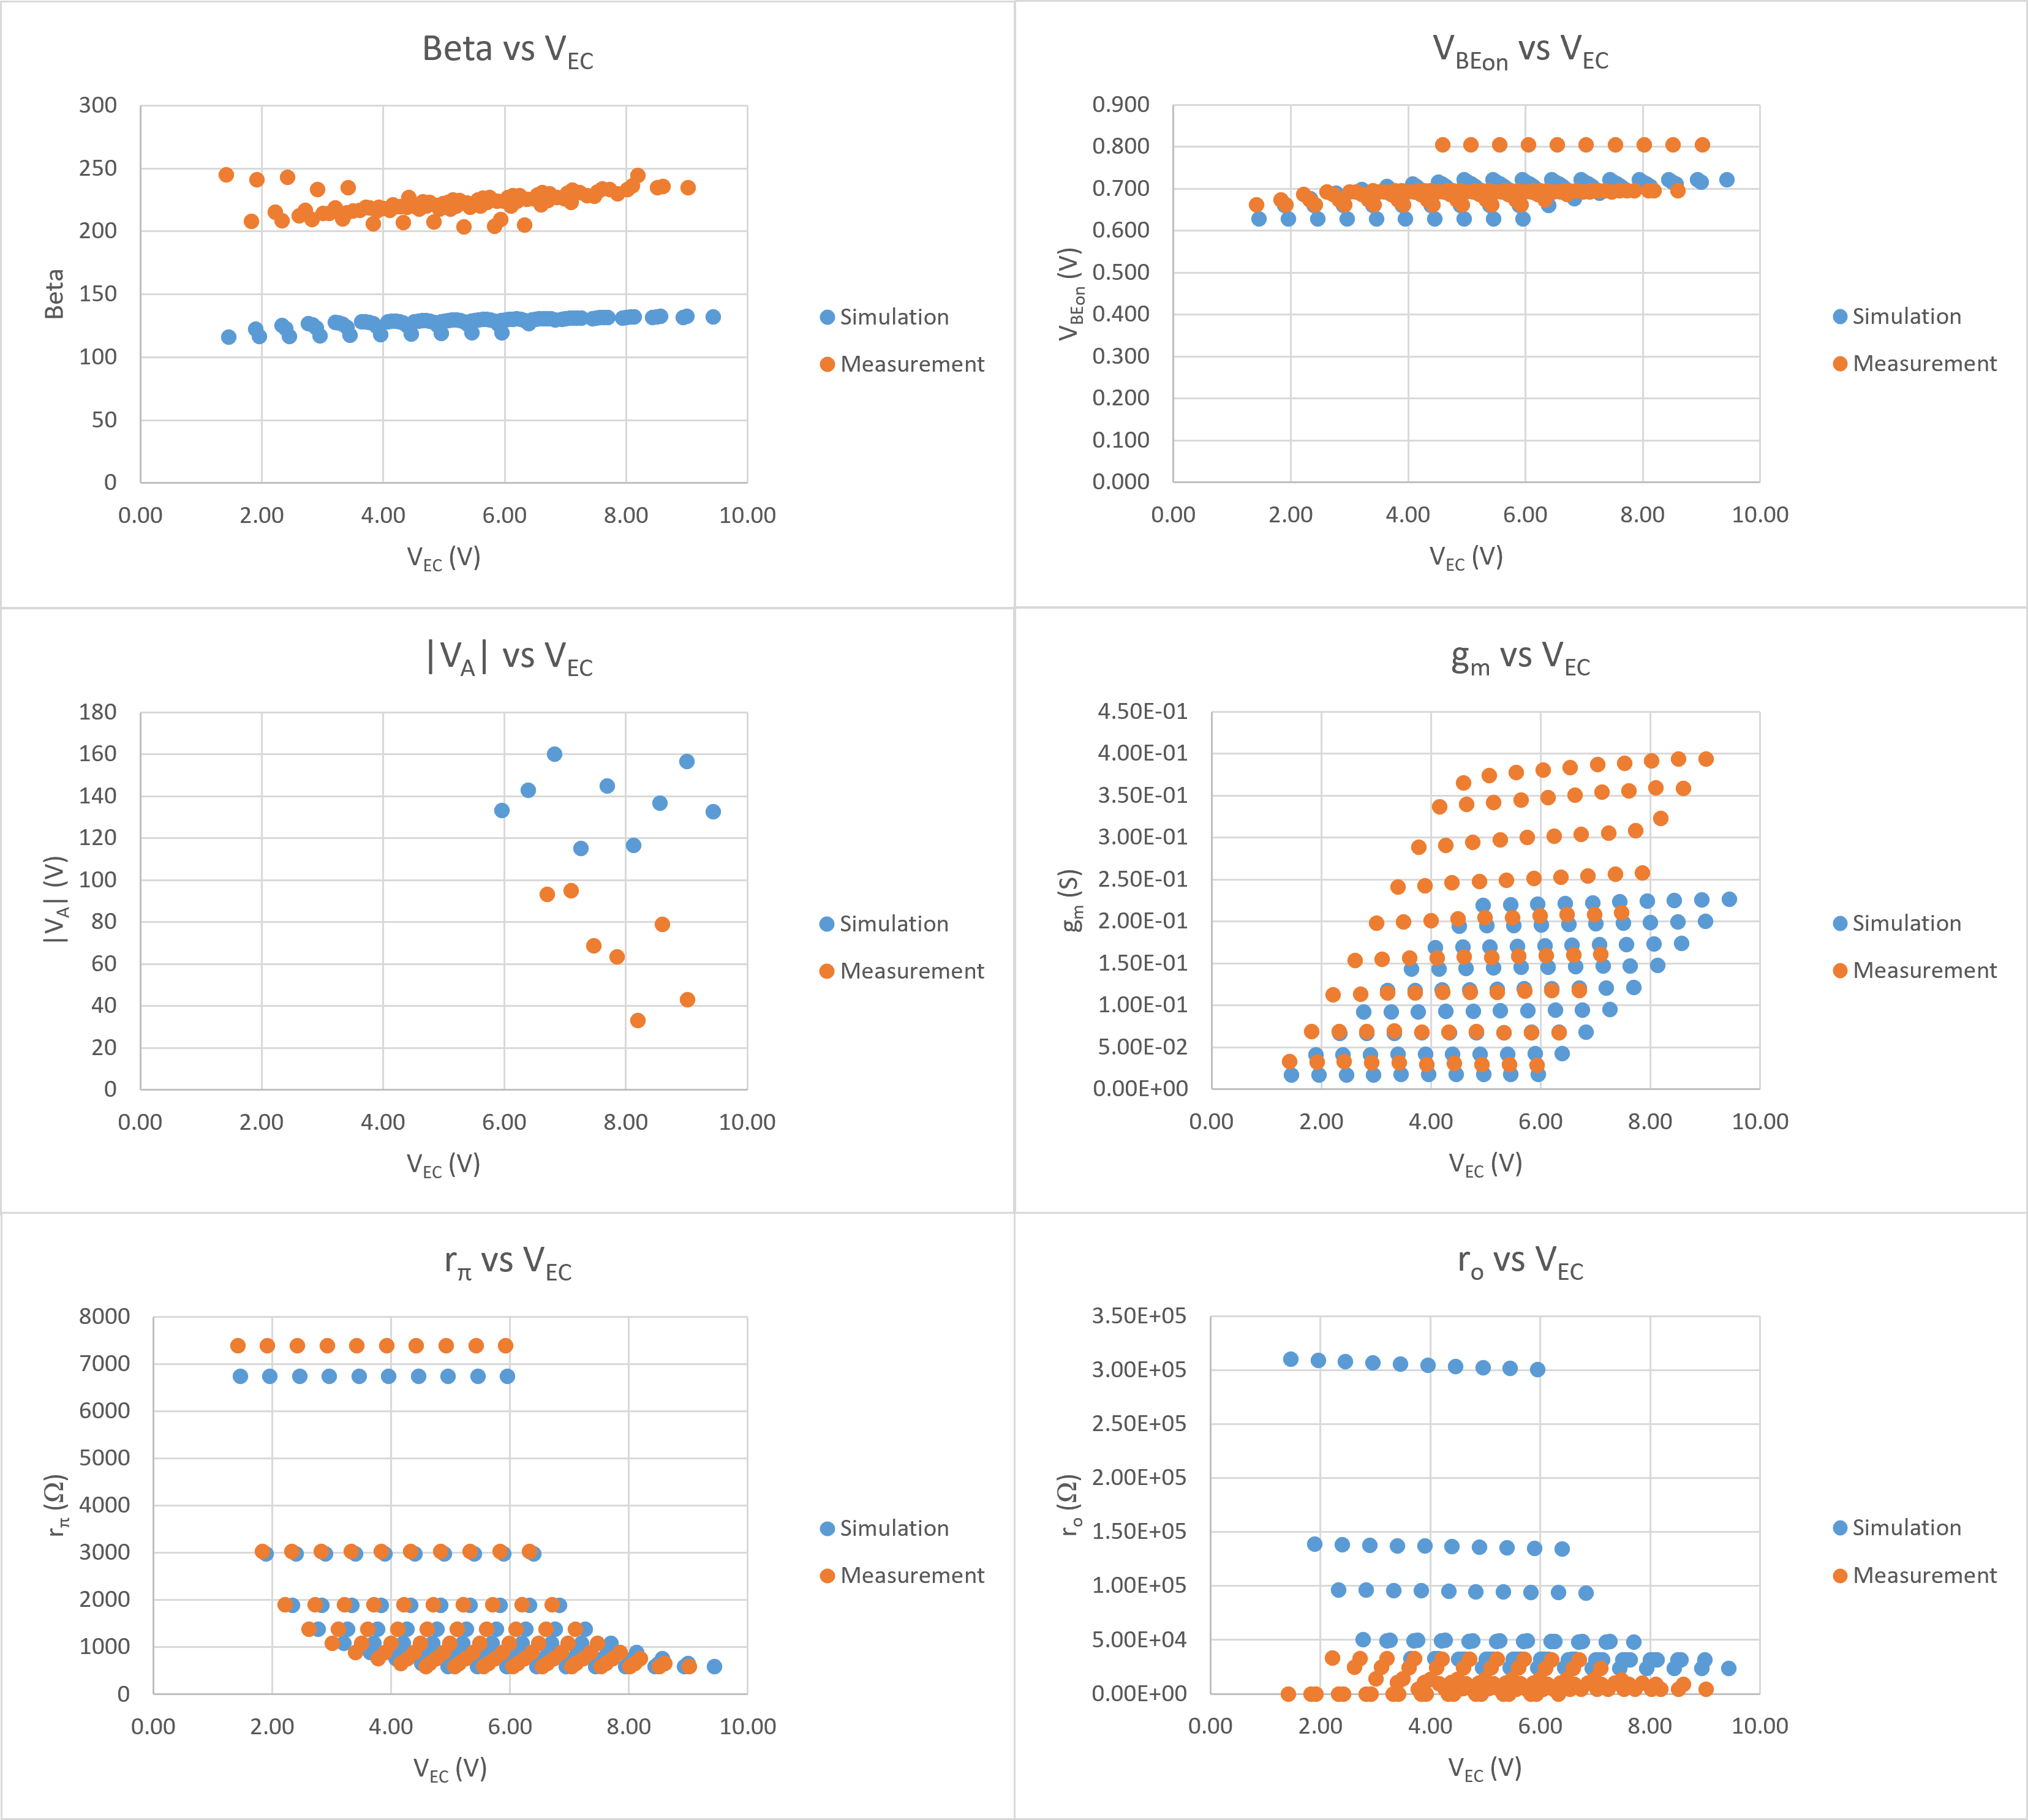
\includegraphics[width=\textwidth]{Q5.png}
        \caption{$\beta$, $V_{EB_{on}}$, $|V_A|$, $g_m$, $r_{\pi}$, $r_o$ vs $V_{CE}$ plots for PNP}
        \label{fig:q5}
    \end{figure} \pagebreak
    \item [\textbf{Q6.}]
    In general, there were no discrepancies between the simulated and measured data; they displayed the similar behaviours in the majority of plots in Figures \ref{fig:q4} and \ref{fig:q5}. The only differences were generally slight shifts between the simulated and measured data, which can be due to a number of factors such as tolerances in the physical components and inaccuracies in the measurements taken by the AD2 board. \pagebreak
    \section*{Part 3}
    \item [\textbf{Q7.}]
    \begin{equation*}
    \begin{gathered}
        I_E = I_B + I_C \\
        I_C = \beta I_B \\
        I_E = (1+\beta) I_B \\
        V_{BE} = V_B - V_E \\
        V_B = V_{BB} - I_B R_{BB} \\
        V_E = V_{EE} + I_E R_3 \\
        V_E = V_{EE} + (1+\beta) I_B R_3 \\
        V_{BE} = V_{BB} - I_B R_{BB} - V_{EE} - (1+\beta) I_B R_3 \\
        I_B  R_{BB} + (1+\beta) I_B R_3 = V_{BB} - V_{EE} - V_{BE} \\
    \end{gathered}
    \end{equation*}
    \begin{equation} \label{eq:ib_thev}
        I_B = \frac{V_{BB} - (V_{EE} + V_{BE_{on}})}{R_{BB} + (1+\beta) R_3} \\
    \end{equation}
    \item [\textbf{Q8.}]
    The difference between equation (\ref{eq:ib_thev}) derived in Q7 and the equation (1.3) derived in the pre-lab is the inclusion of $(1+\beta)R_3$ in the denominator. The additional term in the denominator  increases the value of the denominator, leading to changes in the numerator (such as the change in the power supply voltage, $\Delta V_{EE}$) causing smaller changes in the base current, $I_B$.
    \item [\textbf{Q9.}]
    The $\pi$ model for the circuit is shown below in Figure \ref{fig:q9}. The derivation of the output resistance is found below the figure.
    \begin{figure}[ht!]
        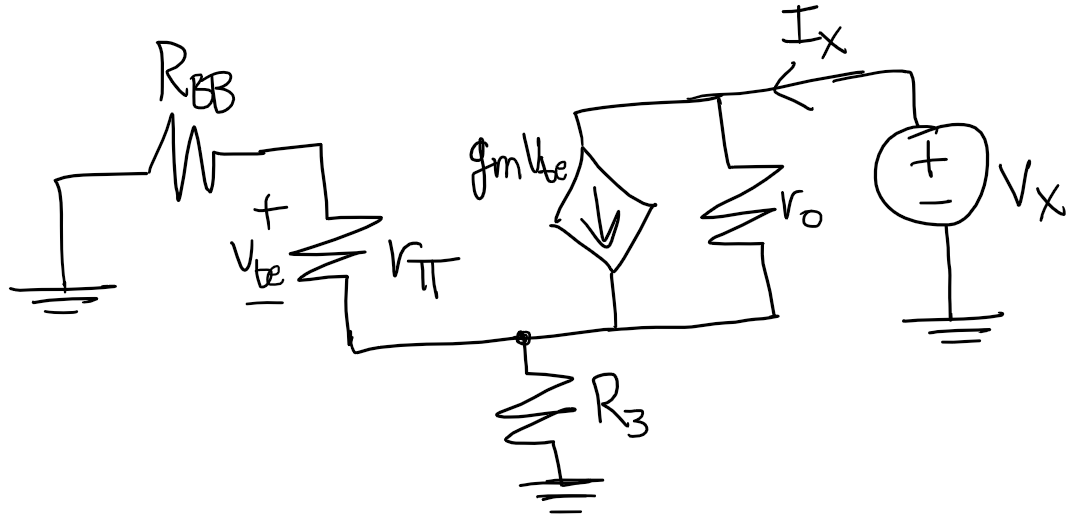
\includegraphics[width=\textwidth]{Q9.PNG}
        \caption{$\pi$ model for circuit}
        \label{fig:q9}
    \end{figure} \\
    \begin{equation*}
    \begin{gathered}
        R_o = \frac{V_x}{I_x} \\
        V_x = (R_3 \parallel (R_{BB}+r_\pi))I_x + (I_x-g_mV_{BE})r_o \\
        V_{BE} = \frac{r_\pi}{R_{BB}+r_\pi}\left[-I_x(R_3 \parallel (R_{BB}+r_\pi))\right] \\
        V_x = (R_3 \parallel (R_{BB}+r_\pi))I_x + (I_x-g_m\left[\frac{r_\pi}{R_{BB}+r_\pi}\left[-I_x(R_3 \parallel (R_{BB}+r_\pi))\right]\right])r_o \\
        V_x = I_x ((R_3 \parallel (R_{BB}+r_\pi)) + r_o + g_mr_o\left[\frac{r_\pi}{R_{BB}+r_\pi}(R_3 \parallel (R_{BB}+r_\pi))\right])
    \end{gathered}
    \end{equation*}
    \begin{equation}
        R_o = \frac{V_x}{I_x} = r_o + \left[R_3 \parallel (R_{BB}+r_\pi)\right] \left[1 + g_mr_o\left(\frac{r_\pi}{R_{BB}+r_\pi}\right)\right]
    \end{equation}
    \item [\textbf{Q10.}]
    To account for the increase in $V_{o,min}$ caused by the insertion of the feedback $R_3$ at the emitter of the BJT, we add the voltage drop across the feedback resistor $R_3$ ($I_E R_3$), to the equation for $V_{o,min}$ provided in the lab.
    \begin{equation}
        V_{o,min} = V_{EE} + I_E R_3 + 0.3
    \end{equation}
    \item [\textbf{Q11.}]
    \begin{equation*}
    \begin{gathered}
        I_o = I_c \\
        V_{o,min} = V_{EE} + I_E R_3 + 0.3 \\
        I_E R_3 = -V_{EE} + V_{o,min} - 0.3 \\
        R_3 = \frac{-V_{EE} + V_{o,min} - 0.3}{I_E} \\
        R_3 = \frac{-V_{EE} + V_{o,min} - 0.3}{I_E} = \frac{-V_{EE} + V_{o,min} - 0.3}{I_o(1+\frac{1}{\beta})}, \beta = 130 \\
        R_3 = \frac{5 - 1 - 0.3 V}{1.0077 mA} \\
        R_3 = \frac{3.7 V}{1 mA} \\
        R_3 = 3.67 k\Omega
    \end{gathered}
    \end{equation*}
    This design was verified on PartSim with a DC sweep of $V_{CC}$ with parameters $R_1 = 40k\Omega$, $R_2 = 500k\Omega$ and $V_{EE} = -5 V$. The simulation active region current sink current was determined to be $997\mu A$, which is extremely close to the targeted value of $1mA$. The simulation plot can be seen in Figure \ref{fig:q11}.
    \begin{figure}[ht!]
        \centering
        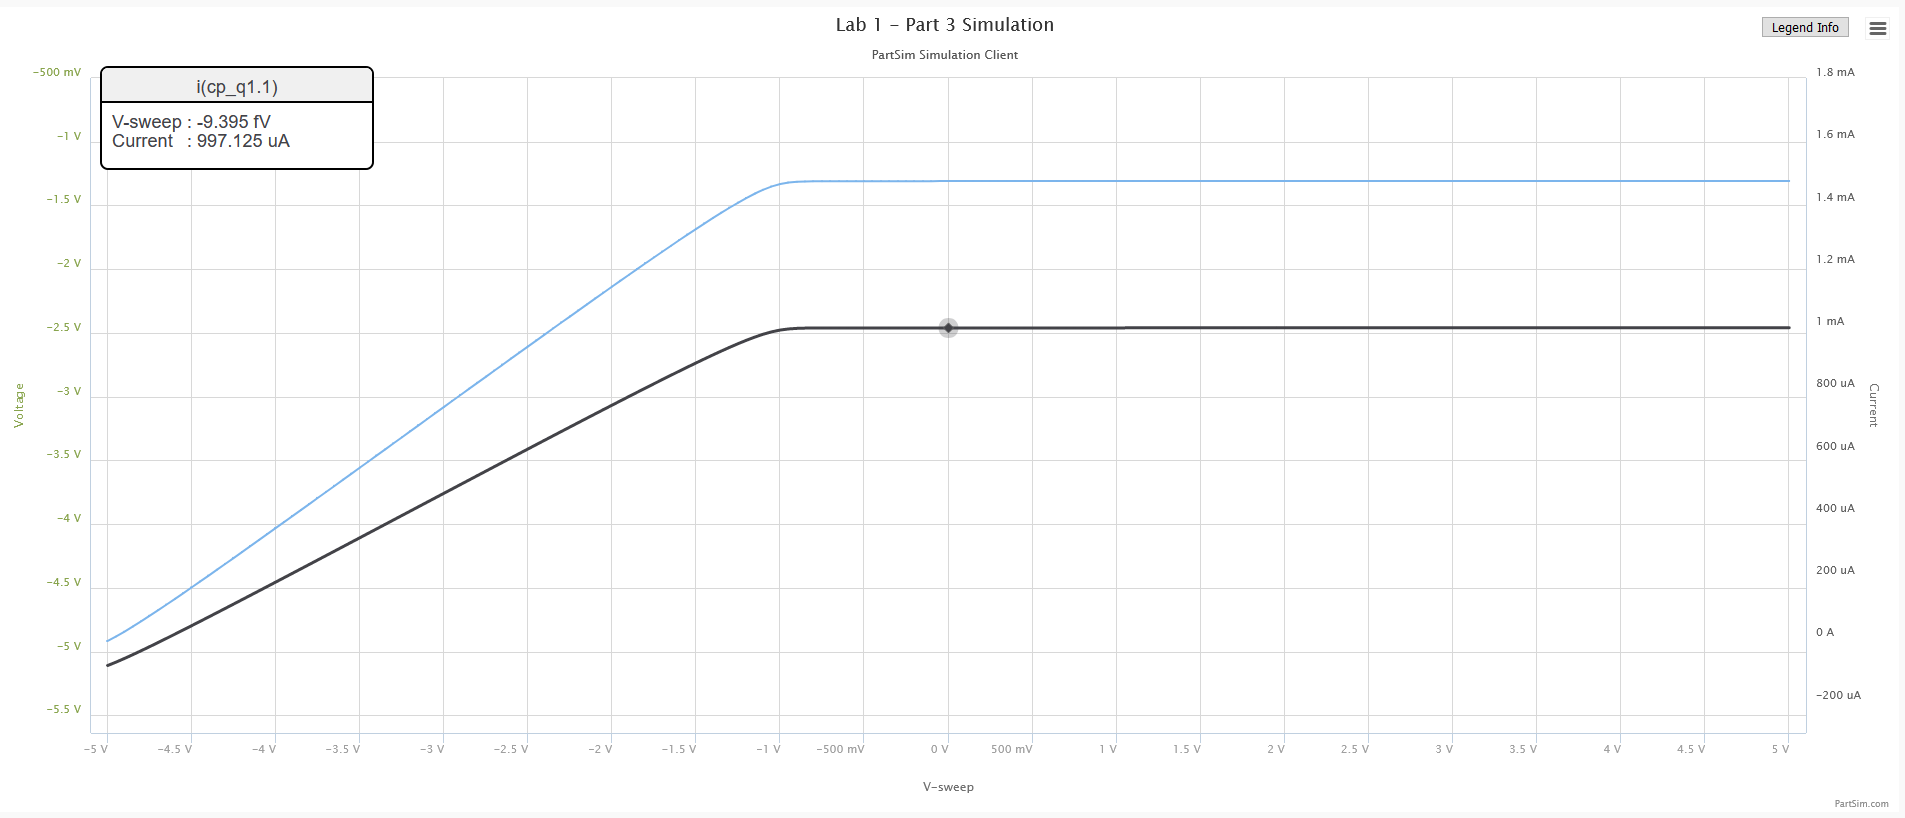
\includegraphics[width=\textwidth]{Q11.png}
        \caption{Plot of designed current sink current, $I_o$, verified to be approximately $1mA$.}
        \label{fig:q11}
    \end{figure} \pagebreak
    \item [\textbf{Q12.}]
    The value of $|V_{CE}|$ required for $Q_1$ to work in the active region was determined by plotting $V_E$ and $I_C$ vs $V_{CC}$ with $R_1, R_2 = 100k\Omega$, $R_3 = 3.67k\Omega$, and $V_{EE} = -5 V$. The active region was determined to have began at approximately $V_{CC} = -2.9 V$, when $V_E = -3.22 V$, this means the value of $|V_{CE}|$ required for $Q_1$ to operate in the active region was determined to be $|V_{CE}| > 0.32 V $. The plots for the simulated $V_E$ and $I_C$ measurements can be seen in Figure \ref{fig:q12}. 
    \begin{figure}[ht!]
        \centering
        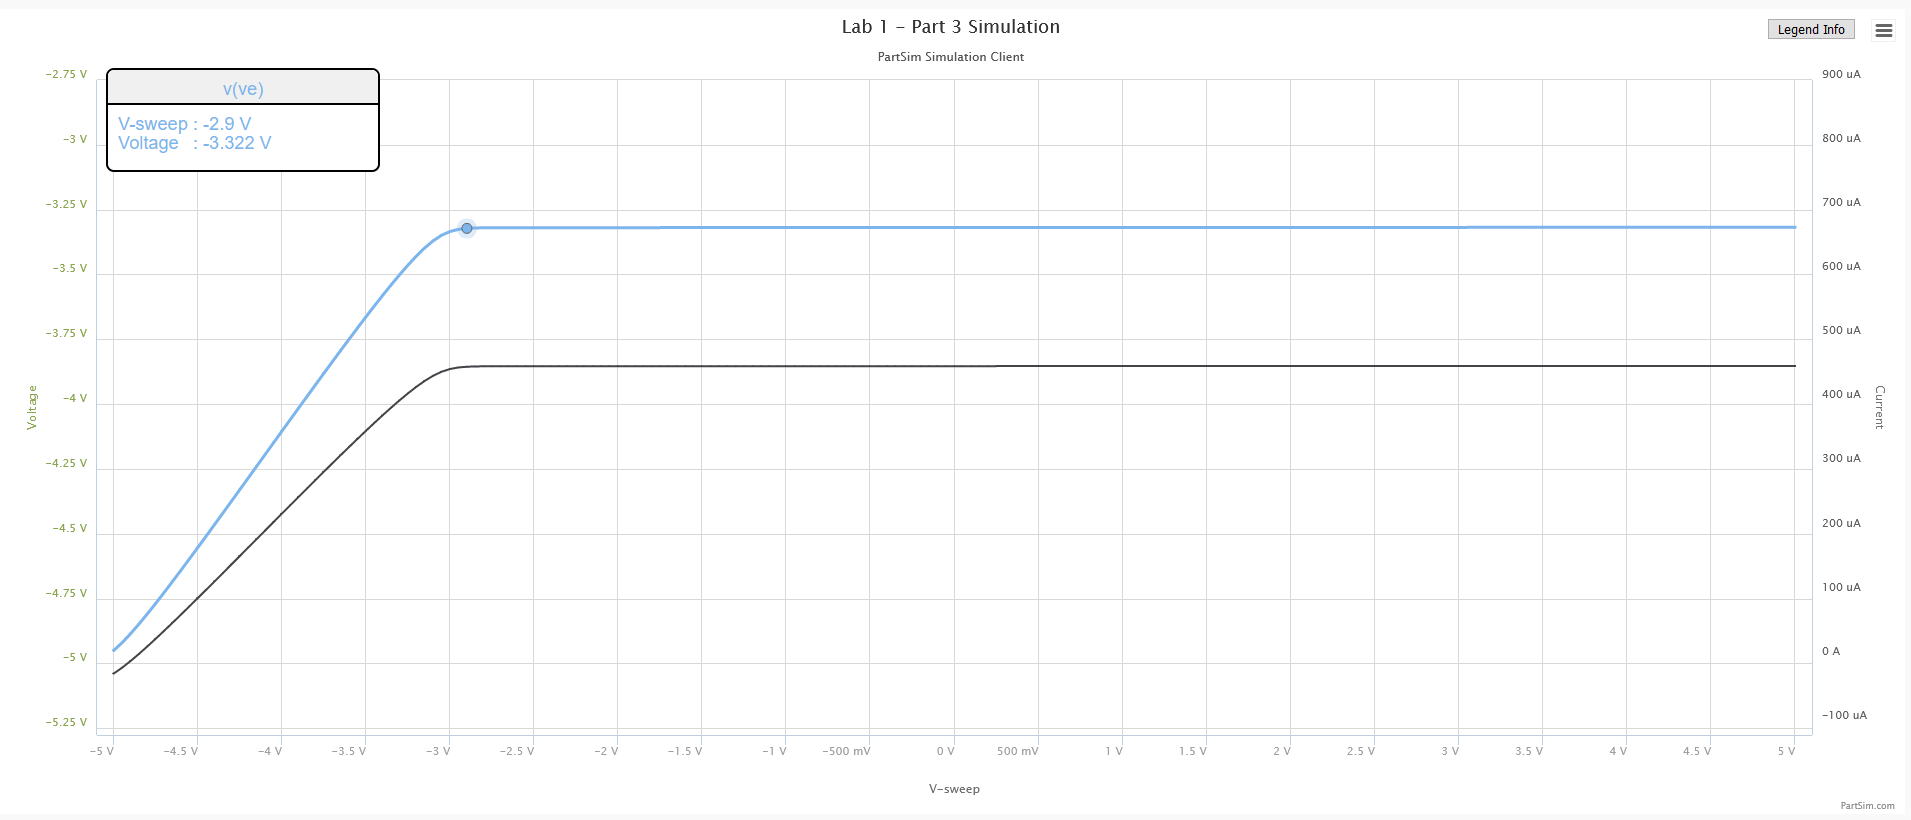
\includegraphics[width=\textwidth]{Q12.png}
        \caption{Plot of $V_E$ and $I_C$ vs $V_{CC}$ for $R_1 = 100k\Omega$, $R_2 = 100k\Omega$, $R_3 = 3.67k\Omega$, $V_{EE} = -5 V$}.
        \label{fig:q12}
    \end{figure}
\end{itemize}
\end{document}